%%==================================================================%%
%% Author : Abascal Fern�ndez, Patricia                             %%
%% Author : S�nchez Barreiro, Pablo                                 %%
%% Version: 1.2, 15/05/2013                                         %%
%%                                                                  %%
%% Memoria del Proyecto Fin de Carrera                              %%
%% Cap�tulo Application Engineering, Archivo ra�z                   %%
%%==================================================================%%

\chapterheader{Ingenier�a de Aplicaci�n}{Ingenier�a de Aplicaci�n}
\label{chap:application}

El cap�tulo anterior describi� el funcionamiento y desarrollo de los generadores de c�digo para la fase de \emph{Ingenier�a del Dominio}. Dichos generadores son los encargados de crear los esqueletos de la implementaci�n de referencia, la cual debe completarse manualmente. Este cap�tulo describe el funcionamiento y desarrollo de los generadores de c�digo para la fase de \emph{Ingenier�a de Aplicaciones}, los cuales tienen como objetivo adaptar la implementaci�n de referencia a las necesidades de cada cliente.

\chaptertoc

\section{Introducci�n}
\label{application:sec:intro}

%%==================================================================%%
%% Author : Abascal Fern�ndez, Patricia                             %%
%% Author : S�nchez Barreiro, Pablo                                 %%
%% Version: 1.2, 24/06/2013                                         %%
%%                                                                  %%
%% Memoria del Proyecto Fin de Carrera                              %%
%% Application Engineering/Introduccion                             %%
%%==================================================================%%

Este cap�tulo describe el proceso de desarrollo de los generadores de c�digo para la segunda fase del desarrollo de una l�nea de productos software (ver Figura~\ref{back:fig:domainAplicEng}), el proceso de \emph{Ingenier�a de Aplicaciones}. El objetivo de esta fase, tal como comentamos, es obtener productos concretos y funcionales a partir de la composici�n, configuraci�n y personalizaci�n de los elementos creados en la fase de \emph{Ingenier�a del Dominio}. 
 
Para ello, de acuerdo con la metodolog�a Te.Net (ver Secci�n~\ref{sec:intr:tenet}), el primer paso es crear una selecci�n de aquellas caracter�sticas que se desea incluir en el producto, de acuerdo a las necesidades particulares de cada clientes. C�mo se crea dicha selecci�n de caracter�sticas est� fuera del �mbito de este proyecto. Referimos al lector interesado al Proyecto Fin de Carrera de D. Daniel Tejedo, antiguo alumno de esta Facultad~\citep{}.

Una vez obtenida una selecci�n de caracter�sticas v�lida, utilizando dicha selecci�n, se configura la arquitectura de referencia creada en la fase de \emph{Ingenier�a del Dominio} para crear un modelo arquitect�nico concreto, adaptado a las necesidades del cliente, del producto que queremos construir.  Dicho modelo arquitect�nico se obtiene de forma autom�tica mediante la utilizaci�n del lenguaje \emph{VML}~\citep{}, de acuerdo con la metodolog�a Te.Net (ver Secci�n~\ref{sec:intr:tenet}). Una descripci�n detallada del lenguaje VML tambi�n est� fuera del �mbito de este proyecto, y referimos al lector interesado a los trabajos de~\cite{} y~\cite{}.

Este modelo arquitect�nico de un product concreto es el que sirve de entrada al generador de c�digo que queremos desarrollar. Utilizando dicho modelo como entrada, el generador de c�digo debe producir todo el c�digo necesario para componer las clases parciales creadas a nivel de \emph{Ingenier�a del Dominio} que correspondan. Para ello debe generar las clases parciales encargadas de llevar a cabo tal composici�n, las versiones limpias de los m�todos requeridos, y las delegaciones a las versiones sucias adecuadas. 

Para ello, el primer paso era dise�ar un algoritmo que permitiese calcular estos tres elementos: (1) clases parciales requeridas; (2) versiones limpias necesarias; y, (3) delegaciones adecuadas. A continuaci�n, deb�amos implementar este algoritmo utilizando plantillas de generaci�n de c�digo, por lo que deb�amos, igual que en cap�tulo anterior, prestar especial atenci�n a su secuenciaci�n. 

Por �ltimo, deb�amos dise�ar y realizar las pruebas que permitiesen comprobar el correcto funcionamiento del generador de c�digo. Tras estas pruebas, se daba por concluido el proceso de desarrollo de los generadores de c�digo, y procedimos a su despliegue. 

Para explicar este proceso de desarrollo, este Cap�tulo se estructura como sigue: La Secci�n~\ref{application:sec:alg} describe la estructura de los modelos de entrada que nuestro generador de c�digo debe procesar. La Secci�n~\ref{application:sec:alg} describe el dise�o del algoritmo encargado de calcular los elementos a componer, de acuerdo al modelo de entrada proporcionado. La Secci�n~\ref{application:sec:transf} explica c�mo se han secuenciado las plantillas de generaci�n de c�digo para poder implementar dicho algoritmo. La Secci�n~\ref{application:sec:pruebas} describe el proceso de dise�o y ejecuci�n de las pruebas para el generador de c�digo implementado. Por �ltimo, la Secci�n~\ref{application:sec:despliegue} detalla las acciones realizadas durante la fase de despliegue de la aplicaci�n.








\section{Configuraci�n de productos a nivel arquitect�nico}
\label{application:sec:mod}

%%==================================================================%%
%% Author : Abascal Fern�ndez, Patricia                             %%
%% Author : S�nchez Barreiro, Pablo                                 %%
%% Version: 1.0, 24/06/2013                                         %%
%%                                                                  %%
%% Memoria del Proyecto Fin de Carrera                              %%
%% Application Engineering/Modelo de Entrada                        %%
%%==================================================================%%

La estrategia para crear un modelo arquitect�nico concreto consiste, tal como se describi� en la Secci�n~\ref{sec:back:uml}, en crear un paquete vac�o, el cual representa el producto a construir, y a�adir relaciones \emph{merge} a aquellas caracter�sticas que se desean incluir en el producto final. De esta forma, el contenido de los paquetes correspondiente a caracter�sticas que se deben incluir en el producto final, se combinan o componen en el paquete que representa el producto final.

Para distinguir el paquete que representa el producto final de los paquetes que representan caracter�sticas, se ha creado un perfil de UML 2.0~\citep{omg:uml:2005}. Un perfil UML 2.0 es un mecanismo gen�rico de extensi�n que permite personalizar los modelos UML para un prop�sito particular, mediante la especificaci�n de estereotipos y valores etiquetados que modifican la sem�ntica original de los elementos del modelo UML 2.0.

\begin{figure}[!tb]
  \center
  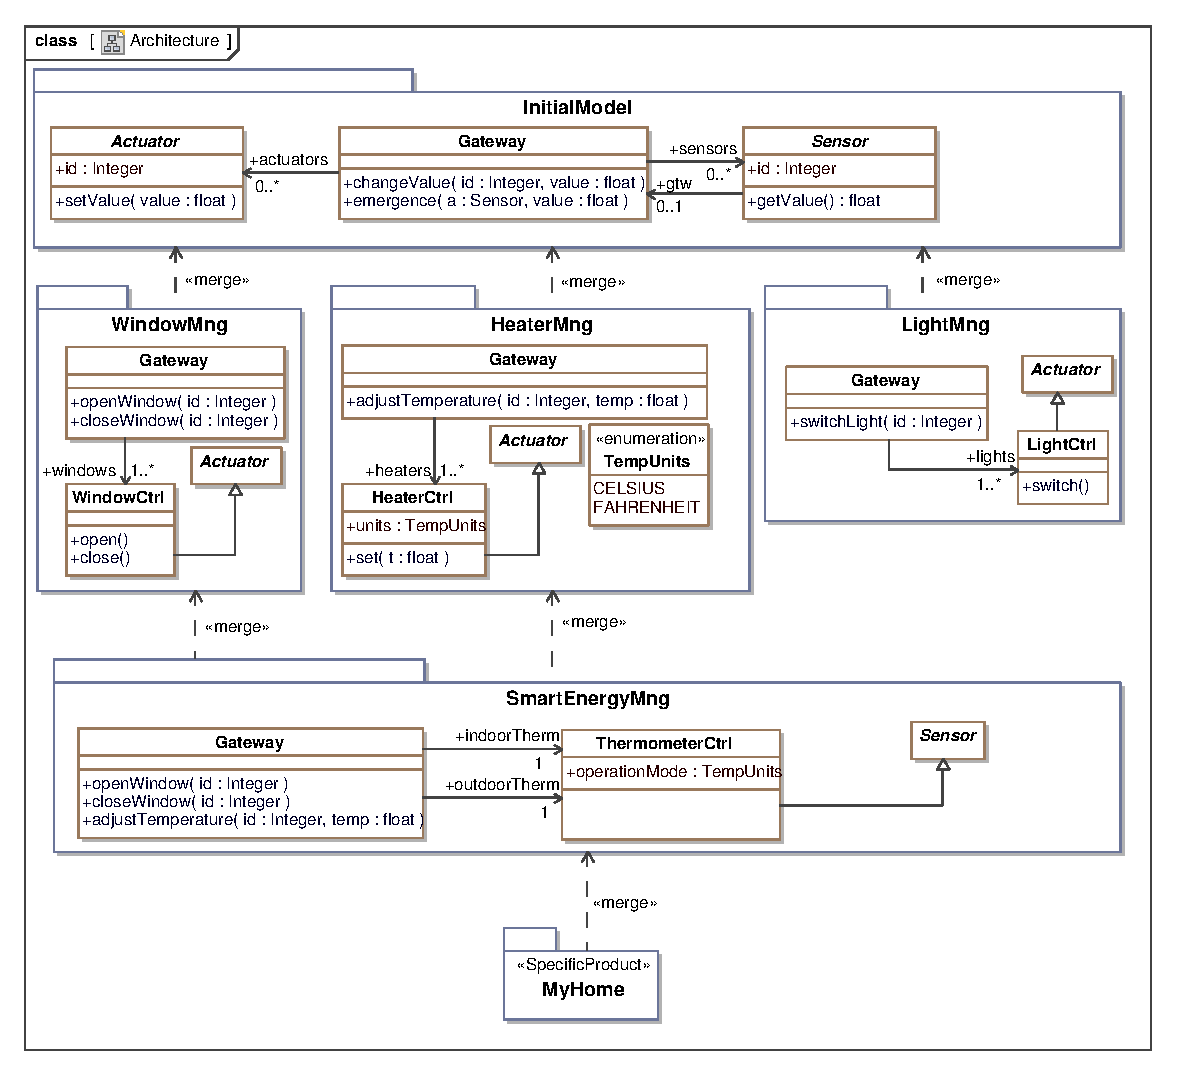
\includegraphics[width=\linewidth]{applicationEngineering/images/Configuration(1).eps} \\
  \caption{Configuraci�n de un hogar inteligente completo}
  \label{app:fig:conf1}
\end{figure}

En nuestro caso, el perfil contiene un solo estereotipo, denominado \imp{SpecificProduct}, el cual se puede aplicar exclusivamente a paquetes UML tal como se puede apreciar en la Figura\ref{app:fig:conf1}. Adem�s, por cada modelo UML 2.0 representando un producto concreto, s�lo puede existir un paquete estereotipado de dicha forma. Esta �ltima restricci�n se expresa por medio de OCL.

La Figura~\ref{app:fig:conf1} muestra un ejemplo de creaci�n de un producto concreto dentro de la l�nea de productos software para hogares inteligentes. En este caso, se trata de un producto donde se ha incluido exclusivamente la caracter�stica de \imp{SmartEnergyMng}, lo que implica que deben seleccionarse adem�s las caracter�sticas \imp{WindowMng} y \imp{HeaterMng}, ya que \imp{SmartEnergyMng} necesita que ambas caracter�sticas est�n instaladas en un producto final para poder funcionar. Dicha dependencia queda especificada de forma expl�cita a trav�s de las relaciones \emph{merge} existentes entre \imp{SmartEnergyMng} y \imp{WindowMng} y \imp{HeaterMng}. Debido a dichas relaciones, es imposible crear un producto que incluya \imp{SmartEnergyMng} pero no \imp{WindowMng} o \imp{HeaterMng}.

La siguiente secci�n describe como este modelo arquitect�nico puede transformarse autom�ticamente en el c�digo necesario para crear una implementaci�n concreta y completamente funcional de un producto software concreto.



\section{Algoritmo para la implementaci�n del producto espec�fico}
\label{application:sec:alg}

%%==================================================================%%
%% Author : Abascal Fern�ndez, Patricia                             %%
%% Author : S�nchez Barreiro, Pablo                                 %%
%% Version: 1.5, 15/05/2013                                         %%
%%                                                                  %%
%% Memoria del Proyecto Fin de Carrera                              %%
%% Application Engineering/Algoritmo                                %%
%%==================================================================%%

Para obtener una implementaci�n completamente funcional de un producto concreto, con unas caracter�sticas determinadas, de acuerdo con el \emph{Slicer Pattern} (ver Secci�n~\ref{sec:back:slicer}), es necesario: (1) crear una clase parcial por cada clase que deba estar incluida en el producto final; (2) crear la \emph{versi�n limpia} de cada constructor y cada m�todo que deba estar incluido en el producto final; y (3) hacer que dichas versiones limpias deleguen en las \emph{versiones sucias} que corresponda.

El primer paso en el proceso de transformaci�n es crear un nuevo proyecto y una nueva carpeta que represente el producto final.

Para calcular todas las clases que deben estar incluidas en el producto final, recorremos el modelo desde el paquete que representa el producto concreto, y que ser� siempre un paquete \emph{hoja}, hacia arriba, hasta llegar a la ra�z, o ra�ces, del modelo orientado a caracter�sticas. Normalmente, siempre hay un modelo ra�z que contiene los elementos que son comunes a todos los productos.
En nuestro caso de la Figura~\ref{app:fig:conf1}, dicho recorrido generar�a dos caminos distintos: (1) \imp{SmartEnergyMng}, \imp{WindowMng}, \imp{BaseSystem}; y (2) \imp{SmartEnergyMng}, \imp{HeaterMng}, \imp{BaseSystem}.

Obviamente, una clase puede aparecer en m�s de un paquete. Por ejemplo, la clase \imp{Gateway} aparece en todos los paquetes, a excepci�n del que representa el producto final, de la Figura~\ref{app:fig:conf1}. No obstante, cada clase que est� en un camino desde el paquete hoja al paquete ra�z, solo debe incluirse una vez en el producto final, aunque �sta aparezca varias veces. Por cada clase distinta presente en algunos de los caminos del paquete hoja a la ra�z, generamos una nueva clase parcial, que colocamos en la carpeta que representa el producto final

A continuaci�n, para cada clase, debemos calcular todos los m�todos limpios que debemos generar. Para ello, al igual que ocurr�a con las clases parciales, recorremos todos los caminos existentes de ra�z a hoja. Para cada clase, por cada m�todo distinto, es decir, con diferente signatura, creamos una versi�n limpia de dicho m�todo dentro de la clase parcial incluida en el producto final. El proceso de generaci�n del esqueleto del m�todo se realiza reutilizando las plantillas de generaci�n de c�digo y facilidades creadas para la Ingenier�a de Dominio.

Por �ltimo, quedar�a por generar el c�digo de cada m�todo, de forma que este delegue en la versi�n sucia del m�todo que corresponda. Es esta fase del algoritmo de generaci�n de c�digo la que entra�a mayor dificultad, porque pueden darse diversos casos. Analizamos cada caso a continuaci�n.

\subsection{Caso 1: S�lo existe una \emph{versi�n sucia} del m�todo}

Se trata del caso m�s simple. S�lo existe una \emph{versi�n sucia} del m�todo, por lo que hay que hacer es delegar en �l. En el ejemplo de la Figura~\ref{app:fig:conf1}, para la clase \imp{Gateway}, el m�todo \imp{WindowCtrl.open}  solo est� implementado en la caracter�stica \imp{WindowMng}, por lo que el c�digo generado para la \emph{versi�n limpia} de dicho m�todo simplemente contendr�a un delegado a la \emph{versi�n sucia} \imp{windowMng\_open} de dicho m�todo.

\subsection{Caso 2: Existen varias \emph{versiones sucias} independientes}

\begin{figure}[!tb]
  \center
  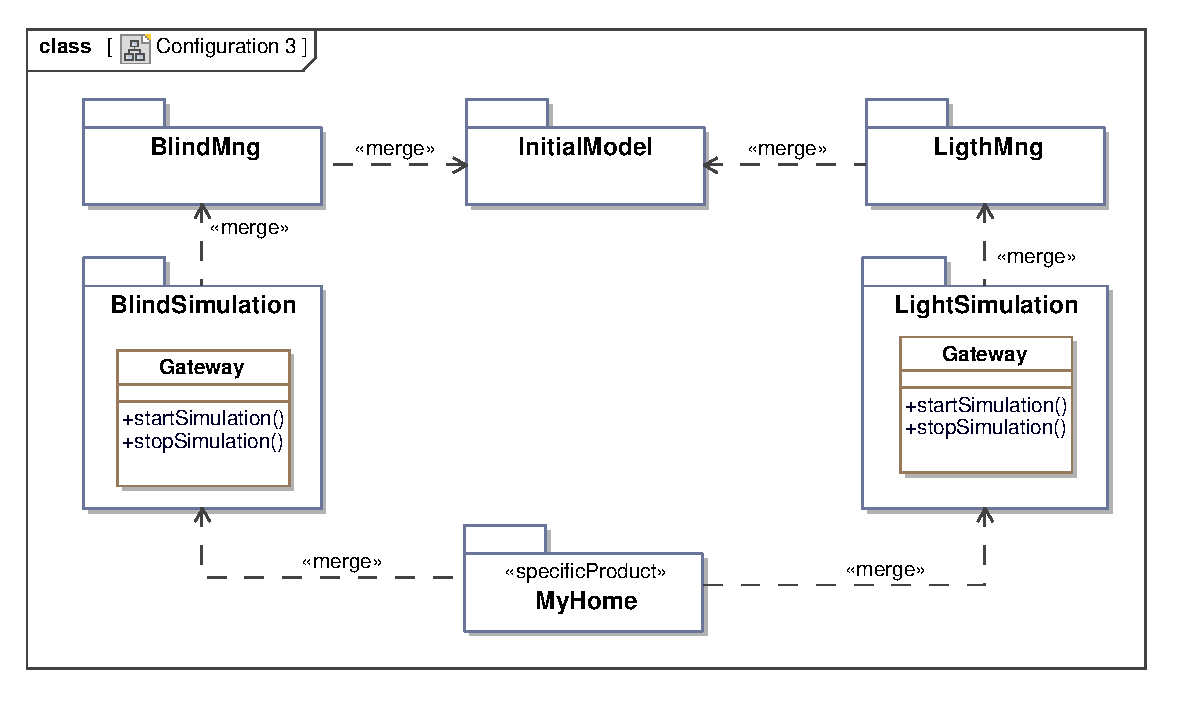
\includegraphics[width=0.80\linewidth,keepaspectratio=true]{applicationEngineering/images/Configuration(2).eps} \\
  \caption{Configuraci�n de una casa inteligente con versiones sucias independientes de un mismo m�todo}
  \label{app:fig:conf2}
\end{figure}

En este caso, existen varias \emph{versiones sucias} independientes del m�todo. Por independientes entendemos que dichas versiones se encuentran en caminos distintos, y ninguna es \emph{alcanzable} desde la otra. El ejemplo de la Figura~\ref{app:fig:conf1} no contiene ninguno de estos casos, por lo que usamos el ejemplo de la Figura~\ref{app:fig:conf2}, extra�do del mismo caso de estudio. Por razones de concisi�n y brevedad, en dicho ejemplo s�lo aparecen aquellos detalles que son relevantes para explicar la situaci�n que estamos tratando.

En este caso, se trata de una configuraci�n de un producto concreto que incluye las caracter�sticas \imp{BlindSimulation} y \imp{LightSimulation}, encargadas de simular la presencia de habitantes en el hogar mediante el movimiento de persianas y el encendido y apagado de luces. Obviamente, ambas caracter�sticas dependen de las caracter�sticas de gesti�n autom�tica de persianas (\imp{BlindMng}) y gesti�n autom�tica de luces \imp{LightMng}, respectivamente. En cada una de estas caracter�sticas, se extiende la clase \imp{Gateway} para que contenga m�todos para iniciar y detener la simulaci�n (\imp{startSimulation} y \imp{stopSimulation}, respectivamente).

En este caso, la versi�n limpia de los m�todos \imp{startSimulation} y \imp{stopSimulation}, contenida dentro del paquete \imp{MyHome}, debe delegar en las versiones sucias del m�todo perteneciente tanto a \imp{BlindSimulation} como \imp{LightSimulation}, ya que en este caso, al inicial la simulaci�n de presencia, deben activarse tanto la simulaci�n de persianas como de luces. Es decir, por ejemplo, el m�todo \imp{startSimulation}, de \imp{MyHome}, contendr� en su interior llamadas a \imp{blindSimulation\_startSimulation} y a \imp{lightSimulation\_startSimualtion}. El orden el cual se generen estas llamadas es irrelevante.

\subsection{Caso 3: Existen \emph{versiones sucias} dependientes de un m�todo}

En este caso, existen varias \emph{versiones sucias} de un m�todo, pero dichas versiones est�n en el mismo camino, estando una situada a mayor profundidad, m�s cerca del paquete \emph{hoja} que la otra. Por ejemplo, en el caso de la Figura~\ref{app:fig:conf1}, existen dos versiones del m�todo \imp{openWindow}, de la clase \imp{Gateway}, en las caracter�sticas \imp{SmartEnergyMng} y \imp{WindowMng}. Ambas est�n en el mismo camino del paquete hoja al paquete ra�z (\imp{SmartEnergy}, \imp{WindowMng}, \imp{BaseSystem}).

En este caso, de acuerdo a la sem�ntica del modelo UML 2.0, la versi�n del paquete \imp{SmartEnergyMng} debe sobrescribir la versi�n del paquete \imp{WindowMng}. Por tanto, la versi�n limpia del m�todo debe invocar en este caso s�lo a la versi�n sucia del paquete \imp{SmartEnergyMng}, ya que se entiende que esta versi�n \emph{m�s profunda} es la m�s actualizada. En caso de haber m�s de dos versiones dependientes, siempre se escoger�a la versi�n m�s profunda.

\subsection{Caso 4: Existen \emph{versiones sucias} dependientes e independientes de un m�todo}

Este caso se trata de una combinaci�n de los casos 2 y 3. Existen diversas versiones de un m�todo. Estas versiones las podemos agrupar en varios subconjuntos, donde cada subconjunto contiene todas las versiones que son dependientes entre s�. Por ejemplo, para la Figura~\ref{app:fig:conf1}, consideremos el caso del constructor de la clase \imp{Gateway}. Supongamos adem�s, que la caracter�stica \imp{LightMng} tambi�n est� seleccionada. Dicho constructor, aunque no se muestra de forma expl�cita en el diagrama, estar�a presente en todas las versiones de dicha clase, presente en cada una de las caracter�sticas del sistema.

Para la Figura~\ref{app:fig:conf1}, hay tres caminos distintos (recordemos que la caracter�stica \imp{LightMng} tambi�n est� seleccionada, aunque no aparezca en la figura): (1) \imp{MyHome}, \imp{SmartEnergyMng}, \imp{WindowMng}, \imp{BaseSystem}; (2) \imp{MyHome}, \imp{SmartEnergyMng}, \imp{HeaterMng}, \imp{BaseSystem}; y, (3) \imp{MyHome}, \imp{LightMng}, \imp{BaseSystem}. En este caso, habr�a 5 versiones del constructor de la clase \emph{Gateway}, m�s concretamente \imp{smartEnergyMng\_Gateway}, \imp{windowMng\_Gateway}, \imp{heaterMng\_Gateway}, \imp{lightMng\_Gateway} y \imp{baseSystemMng\_Gateway}. Tendr�amos dos conjuntos de m�todos dependientes, \{ \imp{smartEnergyMng\_Gateway}, \imp{windowMng\_Gateway}, \imp{heaterMng\_Gateway}, \imp{baseSystemMng\_Gateway} \}, y \{ \imp{lightMng\_Gateway} y \imp{baseSystemMng\_Gateway} \}.

En este caso, la versi�n limpia del m�todo debe invocar la versi�n m�s profunda de cada conjunto independiente de m�todos, en este caso \imp{smartEnergyMng\_Gateway} y \imp{lightMng\_Gateway}. Al igual que en el caso 2, el orden en el cual se invocan estos m�todos es irrelevante.

La siguiente secci�n describe, de forma muy superficial, como se organizan las plantillas encargadas de implementar este no trivial algoritmo de generaci�n de c�digo.


\section{Generadores de C�digo C\#}
\label{application:sec:transf}
%%==================================================================%%
%% Author : Abascal Fern�ndez, Patricia                             %%
%% Author : S�nchez Barreiro, Pablo                                 %%
%% Version: 2.9, 25/04/2013                                         %%
%%                                                                  %%
%% Memoria del Proyecto Fin de Carrera                              %%
%% Domain Engineering/Generadores de C�digo C#                      %%
%%==================================================================%%

Para implementar los generadores de c�digo, se procedi� en encapsular cada una de las reglas descritas en la secci�n anterior en un \emph{template} de EGL. Adem�s, se crearon una serie de funciones auxiliares en EOL. Por ejemplo, se cre� una funci�n auxiliar para determinar el tipo de colecci�n que debe ser utilizada para transformar un atributo multivaluado, es decir, con cota superior de su multiplicidad mayor que uno.

Uno de los mayores problemas que normalmente plantean los generadores de c�digo es que la generaci�n de c�digo es secuencial, no permitiendo la vuelta a atr�s. Por ejemplo, si generamos una clase y m�s tarde descubrimos que dicha clase debe ser modificada porque act�a como clase padre en una herencia m�ltiple, ya no podremos volver a abrir dicha clase para a�adirle la relaci�n de herencia con la interfaz que ha de crearse.

Por tanto, antes de generar una clase, debemos asegurarnos de que no va a necesitar ser modificada posteriormente. Ello implica que hay que tener especial cuidado a la hora de dise�ar el orden en el cual se ejecutan las plantillas, o \emph{templates} de generaci�n de c�digo. La Figura~\ref{dom:fig:templates} muestra el orden de ejecuci�n de las plantillas creadas en nuestro caso. Explicamos parte de dicha figura, aunque no la describiremos entera, por razones de espacio.

\begin{figure}[!tb]
  \centering
  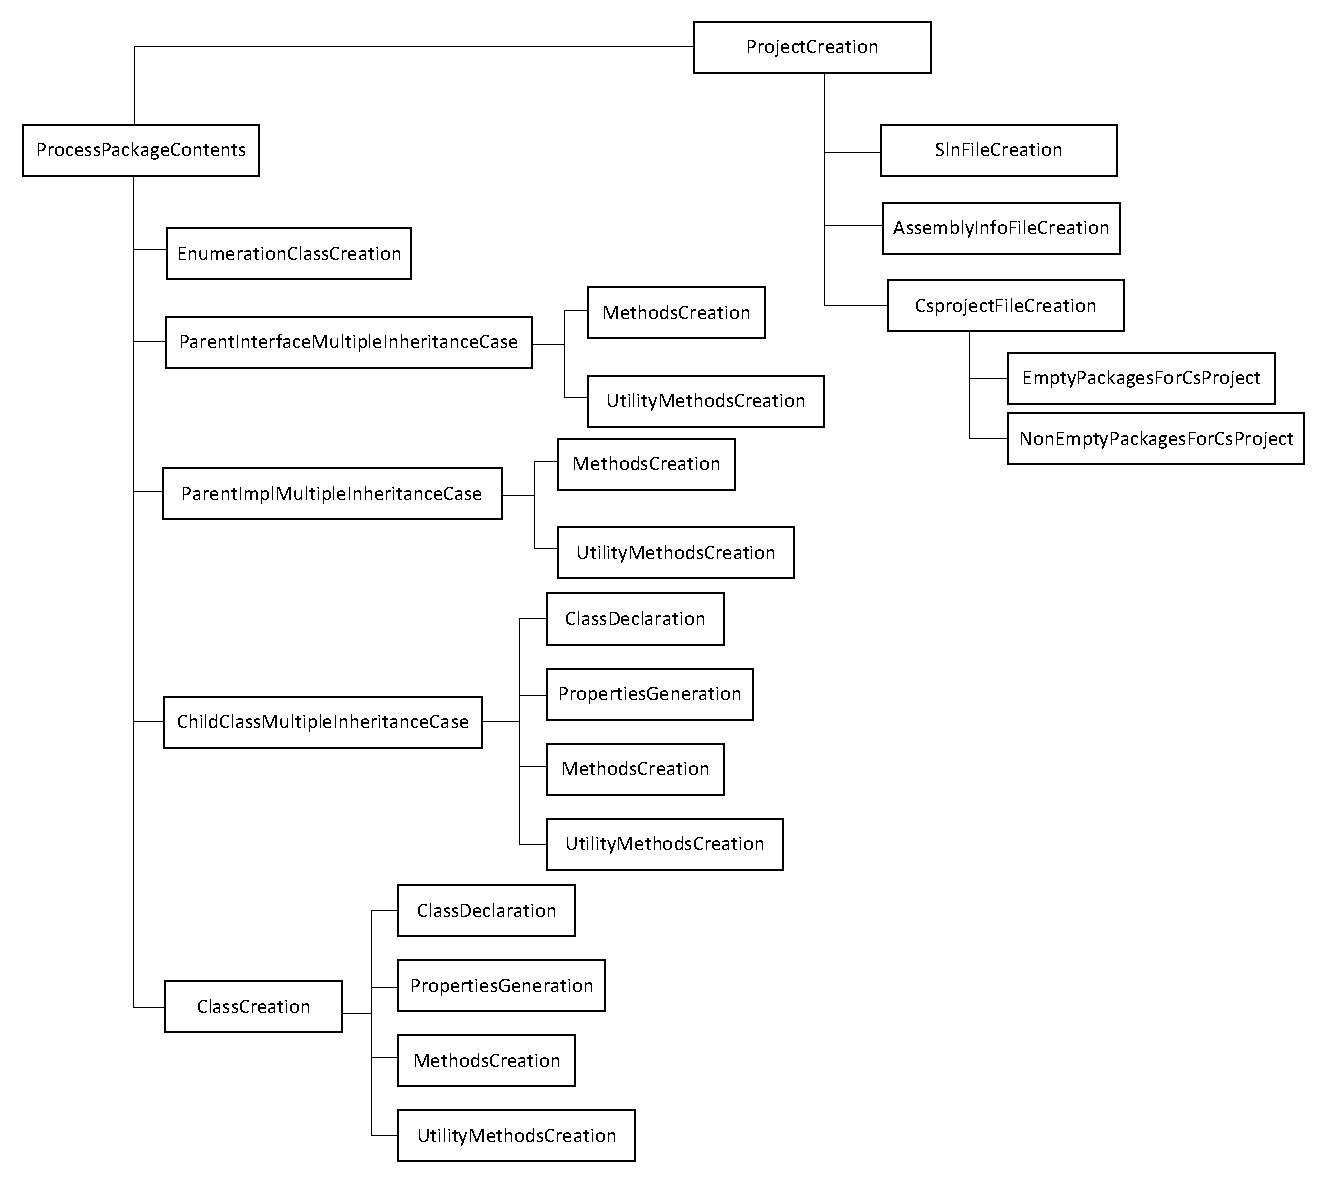
\includegraphics[width=0.9\linewidth]{domainEngineering/images/Templates.eps} \\
  \caption{Orden de ejecuci�n de las plantillas de generaci�n de c�digo}
  \label{dom:fig:templates}
\end{figure}

El punto de partida es el generador de c�digo llamado \imp{ProjectCreation}, encargado de procesar el elemento \emph{modelo}, que constituye la ra�z del proyecto, as� como los \emph{paquetes} que contiene dicho modelo, adem�s de crear el proyecto \emph{Visual Studio 2010} que constituye la salida del generador.  Dicho \emph{template} tiene , por tanto, dos tareas claramente diferenciadas: (1) por una parte, debe generar el c�digo correspondiente a la arquitectura de referencia, lo que se hace a trav�s de la plantilla \imp{ClassFilesCreation}; y (2) por otra parte, debe generar todos los ficheros auxiliares y la estructura que constituyen un proyecto \emph{Visual Studio 2010}, como el fichero de construcci�n (fichero \emph{.csproj}) que indica que clases parciales deben compilarse cuando se construye el proyecto (ver Figura~\ref{back:code:partialClasses}). Para generar estos ficheros auxiliares, se utilizan las plantillas \imp{SlnFileCreation},  \imp{CsprojectFileCreation} y \imp{AssemblyInfoFileCreation}.

La plantilla \imp{ProcessPackageContents} procesa por cada paquete, su contenido. Dependiendo del tipo de cada elemento, se realiza una acci�n diferente, tal como se describe a continuaci�n.

Si se trata de una clase enumerada, se invoca el template \imp{EnumerationClassCreation}, con dicho elemento como argumento.

Se procesan todas las clases con herencia m�ltiple, para aplicar el \emph{mixin pattern}. Para ello se ejecutan las plantillas \imp{ParentImplMultipleInheritanceCase}, que se encarga de procesar las clases padre involucradas en herencias m�ltiples; y \imp{ParentInterfaceMultipleInheritanceCase}, que se encarga de crear las interfaces para estas clases padre. Ambas plantillas hacen uso de las plantillas \imp{MethodsCreation} y \imp{UtilityMethodsCreation}, encargadas de procesar los m�todos de dichas clases e interfaces y de crear los m�todos de infraestructura que fuesen necesarios, tal como \imp{Equals} o \imp{CompareTo}.

A continuaci�n, se ejecuta la plantilla \imp{ChildClassMultipleInheritance}, encargada de procesar una clase hija involucrada en herencia m�ltiple. Para ello se procesan el esqueleto de la clase (\imp{ClassDeclaration}), sus atributos (\imp{PropertiesGeneration}), sus m�todos (\imp{MethodsCreation}) y sus m�todos de infraestructura (\imp{UtilityMethodsCreation}).

Seguidamente, se procesan las clases no afectadas, como hijas o como padres, por herencia m�ltiple. Estas clases se procesan a trav�s de la plantilla \imp{ClassCreation}, que funciona igual que la plantilla \imp{ChildClassMultipleInheritance}, a excepci�n de que no se genera el c�digo de los delegados para los \emph{mixins}.

\begin{figure}[!tb]
  \center
  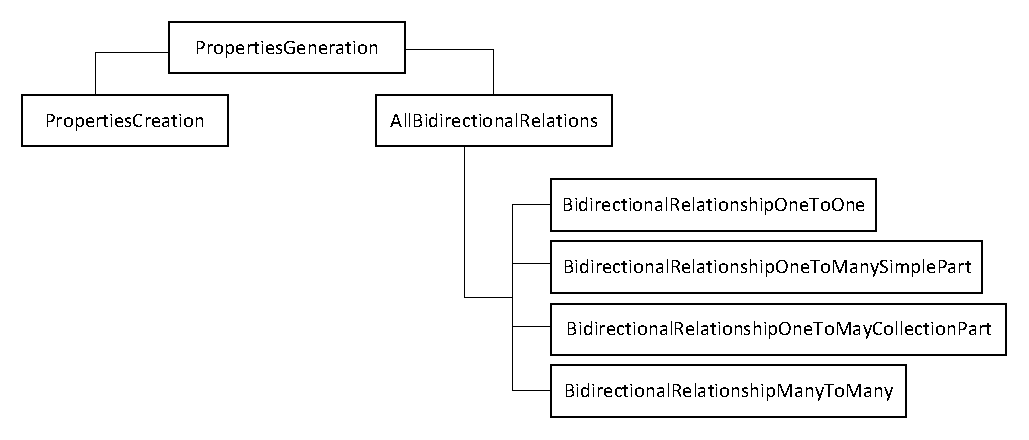
\includegraphics[width=\linewidth]{domainEngineering/images/PropertiesTemplates.eps} \\
  \caption{Orden de ejecuci�n en la plantilla de generaci�n de c�digo \imp{PropertiesGeneration}}
  \label{dom:fig:propTemp}
\end{figure}

Cada plantilla invocada hace uso a su vez de otras subplantillas, que por razones de claridad y espacio no detallamos. Por ejemplo, la plantilla \imp{PropertiesGeneration} encargada de procesar atributos y extremos de asociaci�n, hace uso de diversas plantillas para procesar los extremos pertenecientes a asociaciones doblemente navegables, tal como se indica en la Figura~\ref{dom:fig:propTemp}.

Por �ltimo, comentar que todas las plantillas utilizan diversas funciones auxiliares especificadas en EOL. Por e

\section{Pruebas}
\label{application:sec:pruebas}
%%==========================================================================%%
%% Author : Abascal Fern�ndez, Patricia                                     %%
%% Author : S�nchez Barreiro, Pablo                                         %%
%% Version: 1.1, 15/05/2013                                                 %%
%%                                                                          %%
%% Memoria del Proyecto Fin de Carrera                                      %%
%% Application Engineering/Pruebas                                          %%
%%==========================================================================%%

Una vez implementados los generadores de c�digo para la fase de \emph{Ingenier�a de Aplicaciones}, el siguiente paso era dise�ar y ejecutar las pruebas necesarias que permitiesen comprobar el correcto funcionamiento de estos generadores. Para dise�ar las pruebas,  siguiendo el mismo procedimiento que en el caso anterior, utilizando la t�cnica de clases de equivalencia y valores l�mites, para luego completar con casos espec�ficos que permitiesen alcanzar el 100\% de la cobertura.  

A diferencia de la fase de \emph{Ingenier�a del Dominio}, en esta fase no se utiliz� \emph{EUnit} para ejecutar dichas pruebas, ya que dicha herramienta no se ajustaba a nuestras necesidades. Por tanto, se crearon los casos de prueba y se ejecutaron a mano, analizando de forma tambi�n manual si la salida producida coincid�a con la esperada. La Tabla~\ref{app:table:pruebas} muestra algunos de los casos de prueba ejecutados.

\begin{table}
\begin{small}
\begin{tabularx}{\linewidth}{|X|l|}
 \hline
{Casos v�lidos}&{Casos no v�lidos} \\ \hline
Configuraci�n con un solo camino hoja-raiz & Paquetes recursivos. \\
Configuraci�n con varios caminos y todos los m�todos independientes &\\
Configuraci�n con varios caminos y alg�n m�todo dependiente &\\
Configuraci�n con varios caminos, donde alg�n m�todo tiene versiones dependientes e independientes &\\
\hline
\end{tabularx}
\end{small}
\caption{Casos de prueba para la fase de Ingenier�a de la Aplicaci�n}
\label{app:table:pruebas}
\end{table}%

Una vez creados y probados los generadores de c�digo, el siguiente paso era empaquetarlos para posibilitar su distribuci�n y uso. La siguiente secci�n describe como se realiza dicha fase de despliegue.
Tras ejecutar estos casos de prueba y comprobar que los generadores de c�digo funcionaban correctamente, d�bamos por concluida la labore de desarrollo de los generadores de c�digo, restando solo su empaquetado y despliegue.



\section{Despliegue}
\label{application:sec:despliegue}
%%==================================================================%%
%% Author : Sa�udo Olmedo, Ignacio                                  %%
%% Author : S�nchez Barreiro, Pablo                                 %%
%% Version: 1.5, 15/05/2014                                         %%
%%                                                                  %%
%% Memoria del Proyecto Fin de Carrera                              %%
%% m2t/Sumario                                                      %%
%%==================================================================%%

Durante este cap�tulo se ha descrito el proceso de desarrollo del generador de c�digo. En primer lugar se ha presentado el c�digo del generador de c�digo y parte de la sintaxis utilizada para construirlo as� como la descripci�n de su realizaci�n. A continuaci�n se ha descrito el proceso de transformaci�n del caso de estudio introducido en el cap�tulo dos. Finalmente se han presentado las pruebas realizadas as� comola herramienta utilizada.   

\section{Sumario}
\label{application:sec:sumario}
%%==================================================================%%
%% Author : Abascal Fern�ndez, Patricia                             %%
%%          S�nchez Barreiro, Pablo                                 %%
%% Version: 1.1, 21/06/2013                                         %%
%%                                                                  %%
%% Memoria del Proyecto Fin de Carrera                              %%
%% Antecedentes, Sumario                                            %%
%%==================================================================%%

Durante este cap�tulo se han descrito los conceptos necesarios para comprender el �mbito y el alcance de este proyecto. Se ha descrito el caso de estudio que se utilizar� a lo largo del documento. A continuaci�n, se ha especificado qu� es una l�nea de productos software, el dise�o orientado a caracter�sticas, la metodolog�a TENTE, las limitaciones de las clases parciales en C\#, c�mo pueden resolverse estas limitaciones mediante el uso del \emph{SlicerPattern} y el proceso de generaci�n de c�digo con Epsilon.



